% !TeX spellcheck = de_DE
\documentclass{uebung_cs}
\usepackage{algo121}
\blattname{Wochenplan: Minimale Spannbäume}

%%%%%%%%%%%%%%%%%%%%%%%%%%%%%%%%%%%%%%%%%%%%%%%%%%%%%%%%%%%%%%%%%%%%%%%%%%%%

\begin{document}
\section*{Vorbereitung}
Lies \href{https://jeffe.cs.illinois.edu/teaching/algorithms/book/Algorithms-JeffE.pdf}{Erickson, Kapitel 7} (oder CLRS Kapitel 23) und schau das Video der Woche.

\section*{Dienstag}
\begin{aufgabe}[Algorithmen und Eigenschaften]\label{tue-first}
	Gegeben sei der Graph G in Abbildung~\ref{example_graph}.
	\begin{enumerate}
		\item (\warmup) Führe Kruskals Algorithmus manuell auf G aus.
		\item Führe Prims Algorithmus manuell auf G aus (Startknoten 0). Zeige den Inhalt der Prioritätswarteschlange zu jedem Zeitpunkt der Ausführung.
		\item Zeige \emph{alle} minimalen Spannbäume von G.
		\item Gib einen effizienten Algorithmus an, der einen (nicht notwendigerweise minimalen) Spannbaum berechnet.
	\end{enumerate}
\end{aufgabe}
\begin{figure}[h]
	\begin{center}
		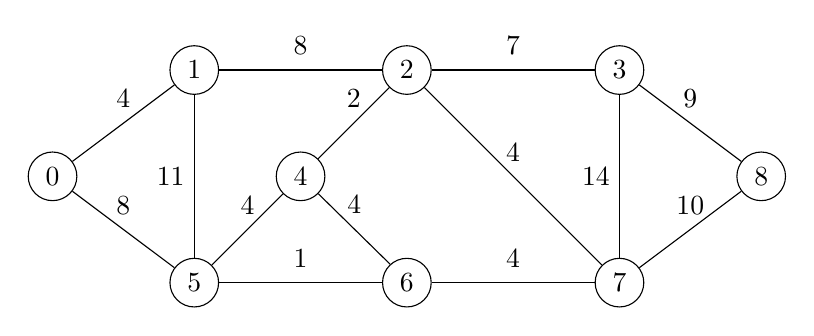
\begin{tikzpicture}[scale=0.9]
			\node[draw,circle] (v0) at (0,  1.5)	{$0$};
			\node[draw,circle] (v1) at (2,  3  )	{$1$};
			\node[draw,circle] (v2) at (5,  3  )	{$2$};
			\node[draw,circle] (v3) at (8,  3  )	{$3$};
			\node[draw,circle] (v4) at (3.5,1.5)	{$4$};
			\node[draw,circle] (v5) at (2,  0  )	{$5$};
			\node[draw,circle] (v6) at (5,  0  )	{$6$};
			\node[draw,circle] (v7) at (8,  0  )	{$7$};
			\node[draw,circle] (v8) at (10, 1.5)	{$8$};
			%
			\def\list {v0/v1/4, v0/v5/8, v1/v2/8, v2/v3/7, v2/v4/2, v2/v7/4, v3/v8/9, v4/v5/4, v4/v6/4, v5/v6/1, v6/v7/4, v7/v8/10}  % list elements
			\foreach \u\v\weight in \list
			{	\draw[-] (\u) -- (\v) node [midway, above=2pt] {\weight};
			}
			\def\vertical {v1/v5/11, v3/v7/14}  % list elements
			\foreach \u\v\weight in \vertical
			{	\draw[-] (\u) -- (\v) node [midway, left] {\weight};
			}
			
			%
		\end{tikzpicture}
		\caption{\label{example_graph}Ein ungerichteter, gewichteter Beispielgraph mit neun Knoten.}
	\end{center}
\end{figure}

\begin{aufgabe}[Kabel für den Riedberg]
	Nach viel hin und her, sowie einigen Planungsfehlern, hat Fachbereich 12 endlich ganze $N$ Gebäude (nummeriert $1,\ldots , N$) am Campus Riedberg fertiggestellt, dabei aber vergessen, Glasfaserkabel verlegen zu lassen.
	Top-Studentin Algolina entwickelt jetzt einen Plan, um alle Gebäude möglichst kostengünstig mit den neusten Glasfaserkabeln miteinander zu verbinden.

	Um zwei Gebäude $B_i$ und $B_j$ mit Glasfaserkabeln zu verbinden, müssen Genehmigungen eingeholt werden, Löcher im Boden gegraben werden, und die Kabel verlegt werden.
	Algolina hat eine Liste mit $M$ Preisen für das paarweise Verbinden zweier Gebäude $B_i$ und $B_j$; Gebäudepaare, die nicht in dieser Liste stehen, können nicht miteinander verbunden werden.
	Die Gebäude zählen als \emph{miteinander verbunden}, wenn es einen Glasfaserkabel-Weg zwischen allen Gebäude-Paaren gibt (es muss also nicht unbedingt eine direkte Verbindung sein).

	Gegeben sei die Liste an Preisen.
	Entwirf einen Algorithmus, der Algolina dabei hilft, den günstigsten Gesamtpreis zu berechnen, bei dem alle Gebäude miteinander verbunden sind.
	Du kannst annehmen, dass es möglich ist, alle Gebäude miteinander zu verbinden.
\end{aufgabe}

\begin{aufgabe}[Graphen kappen]
	Zur Bestimmung eines minimalen Spannbaums wird folgender Algorithmus vorgeschlagen: Starte mit einem gewichteten, zusammenhängenden Graphen~$G$. Betrachte die Kanten von $G$ mit absteigendem Gewicht (vom höchstem zu niedrigstem Gewicht).
	Für jede Kante gilt: Behalte diese Kante, falls das Entfernen dieser Kante den Graphen in zwei Zusammenhangskomponenten aufteilen würde. Entferne sie, falls dies nicht der Fall ist.
	Gib die finale Menge an Kanten zurück.
	\begin{enumerate}
		\item Führe den Algorithmus manuell auf G aus Abbildung~\ref{example_graph} aus.
		\item Argumentiere, warum der Algorithmus immer einen minimalen Spannbaum von $G$ findet.
	\end{enumerate}
\end{aufgabe}

\section*{Donnerstag}
\begin{aufgabe}[Eigenschaften von MSTs]
	Sei $G$ ein gewichteter Graph.
	\begin{enumerate}
		\item Zeige, dass die Kante mit dem geringsten Gewicht in $G$ immer im minimalen Spannbaum von $G$ enthalten ist.
		Wie ist es mit der Kante mit dem höchsten Gewicht? 
		\item Wir skalieren alle Kanten-Gewichte in $G$, indem wir sie mit einem Wert $c>0$ multiplizieren.
		Wie sieht der minimale Spannbaum für den neuen Graphen aus?
		\item Zeige, dass es einen \emph{eindeutigen} minimalen Spannbaum für den Graphen $G$ gibt, wenn alle Kantengewichte verschieden sind.
		\textit{Hinweis: Erinnere dich an die Eigenschaften von minimalen Spannbäumen.}
		\item Kruskals Algorithmus kann verschiedene minimale Spannbäume für einen Graphen $G$ zurückgeben, wenn wir zwei Kanten mit gleichem Gewicht anders sortieren.
		Zeige: Für jeden minimalen Spannbaum $T$ in $G$ gilt, dass es eine Möglichkeit gibt, die Kanten so zu sortieren, dass Kruskals Algorithmus $T$ zurückgibt.
	\end{enumerate}
\end{aufgabe}


\begin{aufgabe}[Maximale Spannbäume]
	Gegeben sei ein gewichteter Graph $G$. Gib einen Algorithmus an, um einen maximalen Spannbaum von $G$ zu bestimmen (also einen Spannbaum mit maximalem Gesamtgewicht).
	\emph{Hinweis: Transformiere das Problem.}
\end{aufgabe}


\begin{aufgabe}[MSTs und kleine Änderungen]
	Wir betrachten nun minimale Spannbäume auf Graphen deren Kantengewichte nicht paarweise verschieden sind.
	\begin{enumerate}
		\item Zeige, dass die Schnitt- und Kreiseigenschaften auch dann gelten, wenn die Kantengewichte nicht eindeutig sind (die Eigenschaften müssen entsprechend umformuliert werden).
		\item Schließe daraus, dass Prims und Kruskals Algorithmus auch in diesem Fall funktionieren.
	\end{enumerate}
\end{aufgabe}

\begin{aufgabe}[MSTs mit kleinen Kantengewichten, \hard]
	Sei $G$ ein gewichteter Graph mit $n$ Knoten und $m$ Kanten, sodass alle Kantengewichte Werte aus der Menge $\{ 1, 2, \ldots , 10\}$ sind.
	Gib einen effizienten Algorithmus an, um einen minimalen Spannbaum von $G$ zu bestimmen.
\end{aufgabe}


\end{document}
